\begin{frame}{Complément}{Essais numériques - prédicteur à 5 points}
    \centering{
    \noindent\color{Primary}\rule{\linewidth}{0.6pt}\\
    \textbf{État initial\\}\color{black}\scriptsize
    \begin{itemize}
        \item Condition de Naumann,
        \item $\varepsilon = 5\,10^{-7}$,
        \item Niveaux 12 à 4, $\Delta x = 40/2^{12} \approx 9 \, 10^{-3}$,
        \item Comparaison à une solution convergée en temps $\Delta t = 10^{-7}$.
    \end{itemize}
    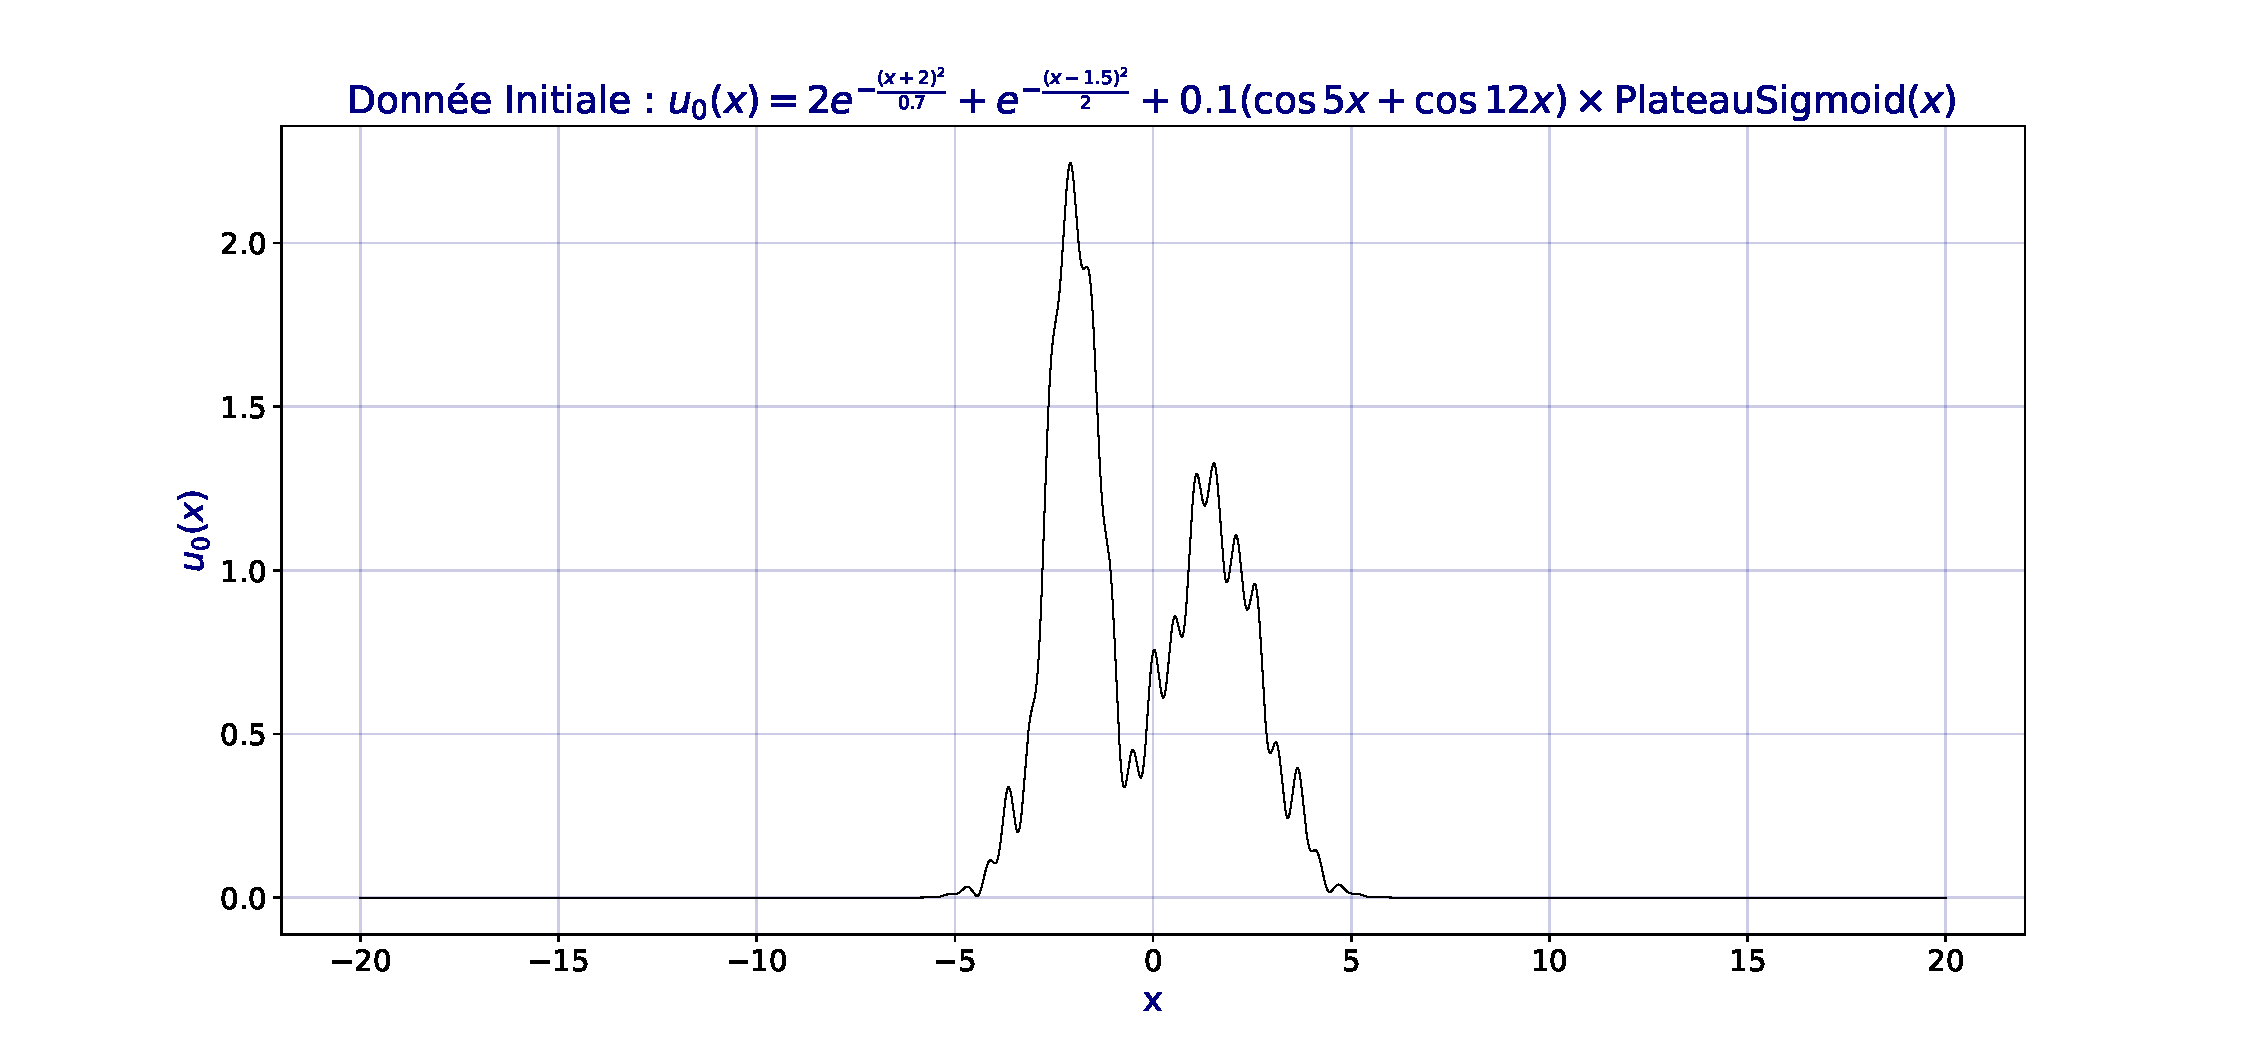
\includegraphics[width = .85\textwidth]{medias/3_/cas_test.pdf}}
\end{frame}